\section{Qualitative Dyanmic For CMS}
\subsection{Qualtiative Mechanical Theory}
The Qualitative Control Theory is a mathematical description of the MCT
In qualitative control theory the  basic patterns of motion are called \textbf{motion primitive}.
In mathematic terms, motion primitives are \textbf{structural stable autonomous systems}

\subsubsection{Basic Concepts of Qualitative Dynamics} 
Qualitative Dynamics can be traced back to Poincare\citep{Poincar'e1899,Poincar'e1885} and recently developed by the Smale School.
Please refer to other books and lectures  such as \citep{abraham1978foundations}for introduction in details.

The configuration of system is described using state value in the state space.
we represent the state of a system as a vector $q$,  $M$ is the state space, which is a manifold.
The motion trajectory over time is $q(t)$.
For a dynamic system, $q(t)$ is usually in the form of  ordinary differential equation. 
\begin{equation}
\dot{q}=F_{u}(q)=F(q,u),q\in M
\label{eq:ode}
\end{equation}
where $u$ is the control effort. 
$F$ is determined by the system's natural property.
If $u=0$,  no control effort is applied.
Such systems are \textbf{autonomous systems}.
For every point $q \in M$, 
$F$ and $u$ determines a derivative vector $\dot{q}$. 
All the vectors over the full space of $M$ form the \textbf{vector field} $V$. 
There is a corresponding geometry structure for Equation \eqref{eq:ode}, a differentiable manifold.
The motion trajectory can be found by apply the integral operation on the vector field.
The result trajectory is defined as \textbf{flow} $\Phi$, all the flows form another geometry structure,
the \textbf{phase portrait}, which illustrates all the possible motions of the dynamic system.


On the phase plane,
Flows can only intersect at some special position.


\textbf{Fix Point} The first type of intersection is fix point or equilibrium point~$q_{e}$.
\[
	H(q_{e})=0
\]

\textbf {Period Flow} Another type of intersection is a periodic flow. For any point $q$ on the circle, we have
\[
	H(q(0))=H(q(T))
\]


Intersections like fixed point and are also called \textbf{equlibria}, 

At each \textbf{equilbria}, 
the local space can be divided into three subspace of submanifold: centre submanifold, stable manifold, and unstable submanifold.

\textbf{centre submanifold}
If a flow $\theta$ pass through a point $m$ on centre submanifold $W_{c}$,
flow$\theta$ will remain on the Centre Manifold 
\[
\theta_{c}(t) \in W_{c}, t \in R
\]
 An equilibria must be on center manifold.

 
\textbf{stable submanifold}
For the flow $\theta_{s}$ passes through a point $m$ on stable submanifold $W_{s}$, the flow will finally converge to a nonwandering point on centre submanifold.
\[
\theta_{s}(+\infty)=\theta_{c}
\]

\textbf{unstable submanifold}
For the flow passes through a point $m$ on unstable submanifold $W_{u}$, the flow will be repelled from the nonwandering points on centre manifold.
An alternative perspective is the inverse of the flow converge to nonwandering point. 
\[
\theta_{u}(-\infty)=\theta_{c}
\] 



For nonlinear system, globally, the shape of stable and unstable submanifold may be bending and connect with itself or each other.
The equilibra and its connectivity of sub manifolds form a topological structure.
The phase plane is divide into different regions,result in a cellular structure.
In each region,there is only one attractor, all the flow in this region will converge to the attractor.
and the corresponding region is called \textbf{basin of attraction}.
\subsubsection{Motion Adaptation and Stability}
A mechanical system can be extremely stable without any control effort. 
This kind of stability is rough stability or structure stability \citep{Andronov1937}.
Rough stability or structure stability is determined by the topology structure of the system\citep{Jonckheere1997}.

Motions vary greatly, this makes it difficult to define motion and tell it from another.
In Qualitative Control Theory, motion should be defined by the topological structure of the coresponding differetial equation.
From topology viewport, motion adaptation can be modelled as homeomorphism.
Homeorphic flows can be generated if the differentiable manifolds are homeomorphic, which means they share the same topological structure,but different shape.

Structure stable autonomous systems have the ability to maintain its topology structure under perturbations.
They generated homeorphic flows while keep the qualitative property, thus the resulting motion is adaptive but qualitatively maintained.

In fact, the effects of control and perturbation can be modelled in the same way.
An autonomous dynamic system is represented as,  
\[
\dot{q}=H(q)
\]
Considering the control and perturbation, the system will be changed into
\[
\dot{q}=H^{'}(q)=H(q)+f(q,t)
\]
Where $f(q,t)$ is used to model both the control and perturbation.

Geometrically, the effect of $f(q,t)$ can be seen as a deformation to the trajectory $q(t)$ on the phase plane.
\[
q^{'}=\Theta(q)
\]
such that 
\[
H^{'}(q)=H(\Theta(q))=H(q^{'})
\]


In Qualitative Control Theory, only final motion results are concerned, 
In mathematical viewport, only the attractors of flows are controlled, while the flow itself is not concerned in motion control.
Also, according two the type of attractors, motion can be group into two groups.

\textbf{Discrete Motion}
Such motions have fixed attractors, typical motions include posture control and picking up motion of the arm.

\textbf{Peridotic Motion}
Such motion have periodic attractors, typical motion include walking, running and heartbeating.

Motions are made up of motion primitives.
Neural control system tweaks the basic motion primitives to achieve specific objective.


Qualitative Control Theory preserve the natural motion features.

\textbf{Adaptive}
Using this method, 
different perturbations will result in different motions. 
Motion will vary with the environment change.

\textbf{Efficient}
Motion will be generated passively and follow the least energy path.

\textbf{Agile}
QCT does not rely on high precise calculation.
Topological structure can be manipulated and maintained by some very simple methods.


\subsection{CPG and Entraintment}
In nature, an animal's body and environment can be extremely complex. 
It leads to high dimensional manifolds with complicated topological structure. 
For CMS application, one question is the whether complex system can be controlled with a simple method.
Biology Research suggested that the motion is mainly controlled by the Central Pattern Generator, which is a small autonomous network that generating rhythmic signals.
The existence of CPG is very common, primitive animals like lamprey and fish, to high level animals like bird, mammal and human\citep{Cohen1988}.
The idea of control motion by rhythmic signals can be modelled as entrainment \citep{Gonz'alez-Miranda2004}.
In this section, we provide the understanding of biological entrainment in the viewport of  Qualitative Control Theory.


\subsubsection{The Biological Entraintment}
Entrainment is the phenomenon that two coupled oscillator systems oscillate in a synchronize way. 
Although the mechanism can be very complex, the phenomenon is universal. 
The classic example shows individual pulsing heart muscle cells.
When they are brought close together, they begin pulsing in synchrony. 

Entrainment will happen when coupling two oscillators with similar oscillation frequencies but with very different characteristics. 
A simple explanation is that energy fluctuates between the two oscillating system.

Given two systems,
\[
\dot x=f(x)
\]
\[
\dot y=g(y)
\]
when two oscillation systems couple, the behaviour of both systems will change. 
The coupled system can be presented with the following equation
\begin{eqnarray}
\dot x=f(x)+m*g(y) \label{eq:couple1}\\
\dot y=g(y)+n*f(x) \label{eq:coule2}
\label{eq:couple}
\end{eqnarray}

where $m$,and $n$ are coupling coefficients. 
When $m$ is large, the behaviour of equation\eqref{eq:couple1} is more dominated by the second term $m*g(y)$. 
This can be seen as a forced oscillation system. 
Even $m$ is small, behaviour of equation\eqref{eq:couple1} can be changed qualitatively.
For some cases, stability can be enhanced and chaotic behavior can be suppressed.


The entrainment model can be applied to CMS, if we took the neural oscillator as $f(x)$ and body as the mechanical oscillator $g(x)$.
The properties of mechanical oscillator can be controlled by the oscillation property of the neural system; the oscillation of mechanical system can be controlled by the oscillation of neural system.
If we increase $n$, we can expect that mechanical oscillators shows the behaviour of neural oscillators. 
Entrainment can help to boost the stability of the mechanical oscillation.
When the mechanical oscillation is disrupted but the neural oscillation remains, after the perturbation is removed, the undisrupted neural oscillation can drive the disrupted mechanical oscillation back to normal.



\subsubsection{The Structural Stable Oscillation of the Neural System}
One extensively studied oscillation model is developed by \citet{neurooscillation}. 
The mathematical presentation is as follows:
\begin{eqnarray}
\tau_{1} \dot{x_{1}}&=&c-x_{1}-\beta v_{1}-\gamma [x_{2}]^{+}-\sum_{j}h_{j}[g_{j}]^{+}\\
\tau_{2} \dot{v_{1}}&=&[x_{1}]^{+}-v_{1}\\
\tau_{1} \dot{x_{2}}&=&c-x_{2}-\beta v_{2}-\gamma [x_{1}]^{-}-\sum_{j}h_{j}[g_{j}]^{-}\\
\tau_{2} \dot{v_{2}}&=&[x_{2}]^{+}-v_{2}\\
y_{i}&=&\mbox{max}(x_{i},0)\\
y_{out}&=&[x_{1}]^{+}-[x_{2}]^{+}=y_{1}-y{2}
\label{eq:matsuta}
\end{eqnarray}
where $x$ and $v$ are state variables of the oscillator, $\tau$,$c$,$\beta$,$\gamma$ are parameters of the oscillator.

Matuoka oscillator is an autonomous oscillator; it can begin to oscillator without any control effort.
It is also adaptive; entrainment behaviour can happen between one Matuoka oscillator and different oscillators. 
But because of the nonlinear properties, its behavior is not completely understood. 
Matsuta\citep{Matsuoka1987} explains the adaptive properties from the location of the roots of  characteristic equation. 
Wilimas\citep{Williamson1998} explains the properties in frequency domain.
In our research, we find some important properties of neural oscillator by investigating the phase portrait.


Basically, neural oscillator shows three important properties:

\textbf{Simple Structure}
The topology structure of neural oscillator is simple, 
it includes one  attractive limit circle and one fix repellor.

\textbf{Large Basin of Attraction}
All the simulations we carried out converged to the same limited circle.

\textbf{Fast Converging Speed}
In most of the case, the flow will converge to the limit circle within one period time.

Features above are shown in \figurename \label{fig:matsuta oscilation}.
\begin{figure}[!h]
\centerline{\subfigure[time state]{
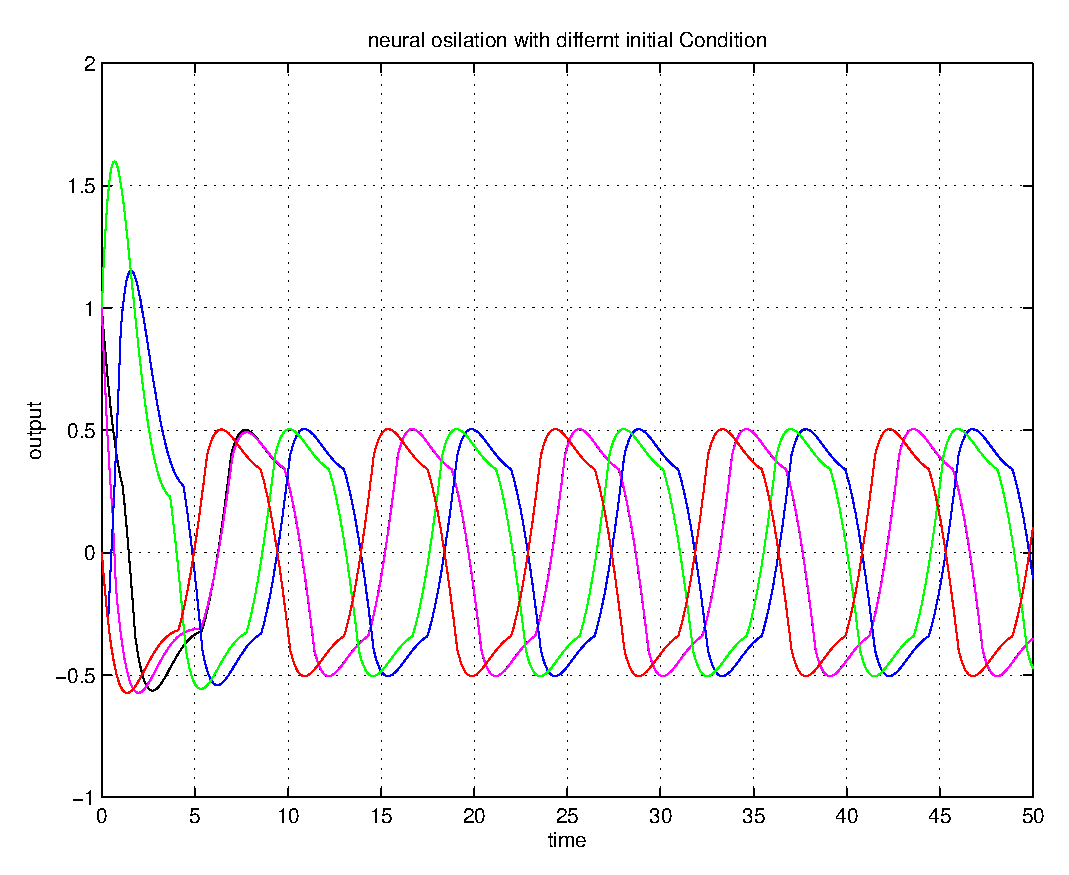
\includegraphics[width=1.5in]{\figurepath/neural_attraction.eps}
\label{fig:time_timeAttraction}
}
\hfill
\subfigure[Phase Portrait]{
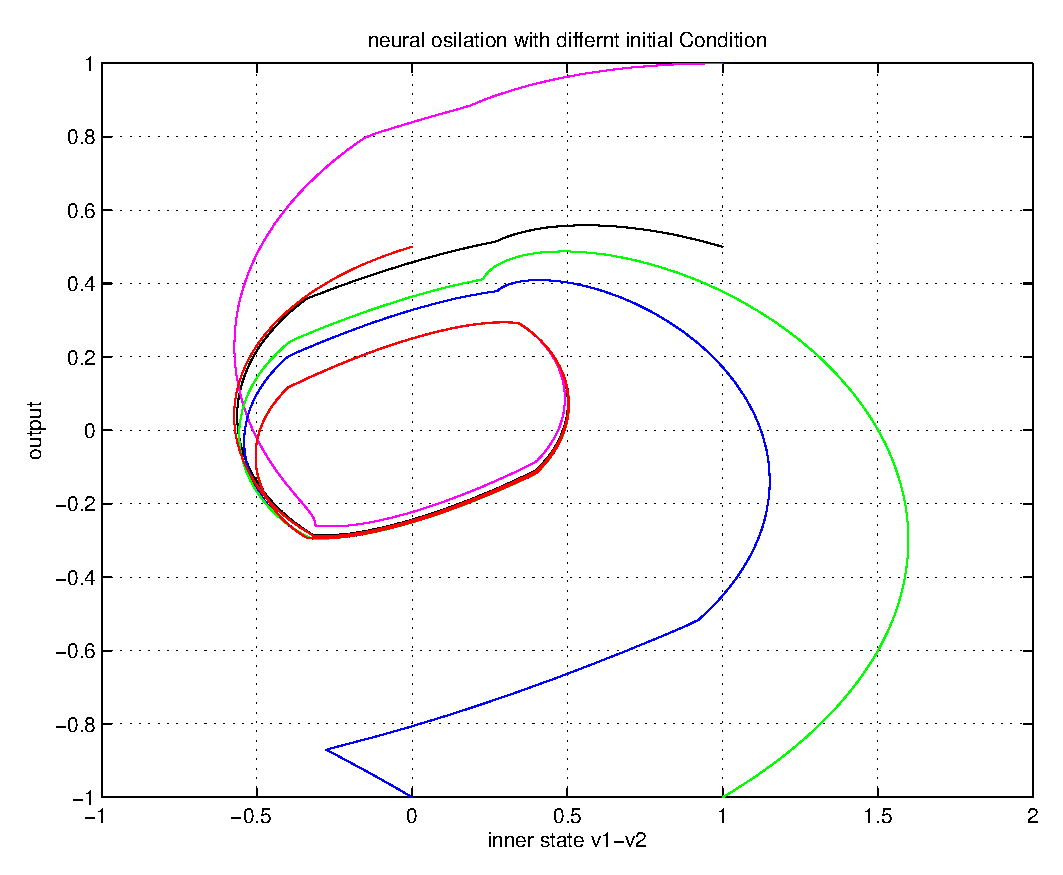
\includegraphics[width=1.5in]{\figurepath/neural_attraction_phase.eps}
\label{fig:phase_attraction}
}
}
\caption{Matsuta Oscilator}
\label{fig:matsuta oscilation}
\end{figure} 
The large area of basin of attraction means the final behavior is totally determined by parameters. 
Initial conditions will have no effects on the final oscillation. 
The converging speed can be seen as quick recovery ability.
When an impulse perturbation happens, it will recover in one period time.
These properties are very valuable in CMS research. 
Matuskota Oscillator is a structure stable autonomous oscillator.
An intuitive idea is that we couple the neural oscillator with mechanical oscillator of body and environment, thus tune the motion a structual stable one
